\documentclass{article}\usepackage[]{graphicx}\usepackage[]{color}
%% maxwidth is the original width if it is less than linewidth
%% otherwise use linewidth (to make sure the graphics do not exceed the margin)
\makeatletter
\def\maxwidth{ %
  \ifdim\Gin@nat@width>\linewidth
    \linewidth
  \else
    \Gin@nat@width
  \fi
}
\makeatother

\definecolor{fgcolor}{rgb}{0.345, 0.345, 0.345}
\newcommand{\hlnum}[1]{\textcolor[rgb]{0.686,0.059,0.569}{#1}}%
\newcommand{\hlstr}[1]{\textcolor[rgb]{0.192,0.494,0.8}{#1}}%
\newcommand{\hlcom}[1]{\textcolor[rgb]{0.678,0.584,0.686}{\textit{#1}}}%
\newcommand{\hlopt}[1]{\textcolor[rgb]{0,0,0}{#1}}%
\newcommand{\hlstd}[1]{\textcolor[rgb]{0.345,0.345,0.345}{#1}}%
\newcommand{\hlkwa}[1]{\textcolor[rgb]{0.161,0.373,0.58}{\textbf{#1}}}%
\newcommand{\hlkwb}[1]{\textcolor[rgb]{0.69,0.353,0.396}{#1}}%
\newcommand{\hlkwc}[1]{\textcolor[rgb]{0.333,0.667,0.333}{#1}}%
\newcommand{\hlkwd}[1]{\textcolor[rgb]{0.737,0.353,0.396}{\textbf{#1}}}%

\usepackage{framed}
\makeatletter
\newenvironment{kframe}{%
 \def\at@end@of@kframe{}%
 \ifinner\ifhmode%
  \def\at@end@of@kframe{\end{minipage}}%
  \begin{minipage}{\columnwidth}%
 \fi\fi%
 \def\FrameCommand##1{\hskip\@totalleftmargin \hskip-\fboxsep
 \colorbox{shadecolor}{##1}\hskip-\fboxsep
     % There is no \\@totalrightmargin, so:
     \hskip-\linewidth \hskip-\@totalleftmargin \hskip\columnwidth}%
 \MakeFramed {\advance\hsize-\width
   \@totalleftmargin\z@ \linewidth\hsize
   \@setminipage}}%
 {\par\unskip\endMakeFramed%
 \at@end@of@kframe}
\makeatother

\definecolor{shadecolor}{rgb}{.97, .97, .97}
\definecolor{messagecolor}{rgb}{0, 0, 0}
\definecolor{warningcolor}{rgb}{1, 0, 1}
\definecolor{errorcolor}{rgb}{1, 0, 0}
\newenvironment{knitrout}{}{} % an empty environment to be redefined in TeX

\usepackage{alltt}
\IfFileExists{upquote.sty}{\usepackage{upquote}}{}
\begin{document}

\begin{knitrout}
\definecolor{shadecolor}{rgb}{0.969, 0.969, 0.969}\color{fgcolor}\begin{kframe}
\begin{alltt}
\hlcom{#GUIA 6}

\hlkwd{getwd}\hlstd{()}
\end{alltt}
\begin{verbatim}
## [1] "C:/Users/Roxy/Documents/ROXANA BEATRIZ RONQUILLO UMA�A/Guias de R"
\end{verbatim}
\begin{alltt}
\hlkwd{setwd}\hlstd{(}\hlstr{"C:/Users/Roxy/Documents/jjjjjjjjjj"}\hlstd{)}
\hlstd{Tipo} \hlkwb{<-} \hlkwd{c}\hlstd{(}\hlstr{"CC"}\hlstd{,} \hlstr{"PC"}\hlstd{,} \hlstr{"SC"}\hlstd{); Tipo}
\end{alltt}
\begin{verbatim}
## [1] "CC" "PC" "SC"
\end{verbatim}
\begin{alltt}
\hlstd{Consumo} \hlkwb{<-} \hlkwd{sample}\hlstd{(Tipo,} \hlnum{20}\hlstd{,} \hlkwc{replace}\hlstd{=}\hlnum{TRUE}\hlstd{); Consumo}
\end{alltt}
\begin{verbatim}
##  [1] "PC" "PC" "SC" "SC" "CC" "PC" "PC" "PC" "CC" "PC" "SC" "PC" "SC" "CC"
## [15] "SC" "SC" "PC" "SC" "CC" "SC"
\end{verbatim}
\begin{alltt}
\hlkwd{data.entry}\hlstd{(Consumo)}
\hlkwd{write}\hlstd{(Consumo,} \hlstr{"Consumo.txt"}\hlstd{)}
\hlkwd{ls}\hlstd{()}
\end{alltt}
\begin{verbatim}
## [1] "Consumo" "Tipo"
\end{verbatim}
\begin{alltt}
\hlkwd{rm}\hlstd{(}\hlkwc{list}\hlstd{=}\hlkwd{ls}\hlstd{(}\hlkwc{all}\hlstd{=}\hlnum{TRUE}\hlstd{))}
\hlkwd{ls}\hlstd{()}
\end{alltt}
\begin{verbatim}
## character(0)
\end{verbatim}
\begin{alltt}
\hlstd{Consumo} \hlkwb{<-} \hlkwd{scan}\hlstd{(}\hlstr{"Consumo.txt"}\hlstd{,} \hlkwc{what} \hlstd{=} \hlkwd{character}\hlstd{(),} \hlkwc{na.strings} \hlstd{=} \hlstr{"NA"}\hlstd{,}\hlkwc{flush}\hlstd{=}\hlnum{FALSE}\hlstd{);Consumo}
\end{alltt}
\begin{verbatim}
##  [1] "PC" "PC" "SC" "SC" "CC" "PC" "PC" "PC" "CC" "PC" "SC" "PC" "SC" "CC"
## [15] "SC" "SC" "PC" "SC" "CC" "SC"
\end{verbatim}
\begin{alltt}
\hlkwd{ls}\hlstd{()}
\end{alltt}
\begin{verbatim}
## [1] "Consumo"
\end{verbatim}
\begin{alltt}
\hlstd{frec} \hlkwb{<-} \hlkwd{table}\hlstd{(Consumo); frec}
\end{alltt}
\begin{verbatim}
## Consumo
## CC PC SC 
##  4  8  8
\end{verbatim}
\begin{alltt}
\hlstd{prop} \hlkwb{<-} \hlkwd{table}\hlstd{(Consumo)}\hlopt{/}\hlkwd{length}\hlstd{(Consumo); prop}
\end{alltt}
\begin{verbatim}
## Consumo
##  CC  PC  SC 
## 0.2 0.4 0.4
\end{verbatim}
\begin{alltt}
\hlkwd{summary}\hlstd{(Consumo)}
\end{alltt}
\begin{verbatim}
##    Length     Class      Mode 
##        20 character character
\end{verbatim}
\begin{alltt}
\hlkwd{barplot}\hlstd{(frec,} \hlkwc{main}\hlstd{=}\hlstr{"Gráfico de barras"}\hlstd{,} \hlkwc{xlab}\hlstd{=}\hlstr{" Consumo"}\hlstd{,} \hlkwc{col}\hlstd{=}\hlkwd{c}\hlstd{(}\hlstr{"yellow"}\hlstd{,} \hlstr{"white"}\hlstd{,} \hlstr{"red"}\hlstd{),}\hlkwc{sub}\hlstd{=}\hlstr{"Agosto-2012"}\hlstd{)}
\end{alltt}
\end{kframe}
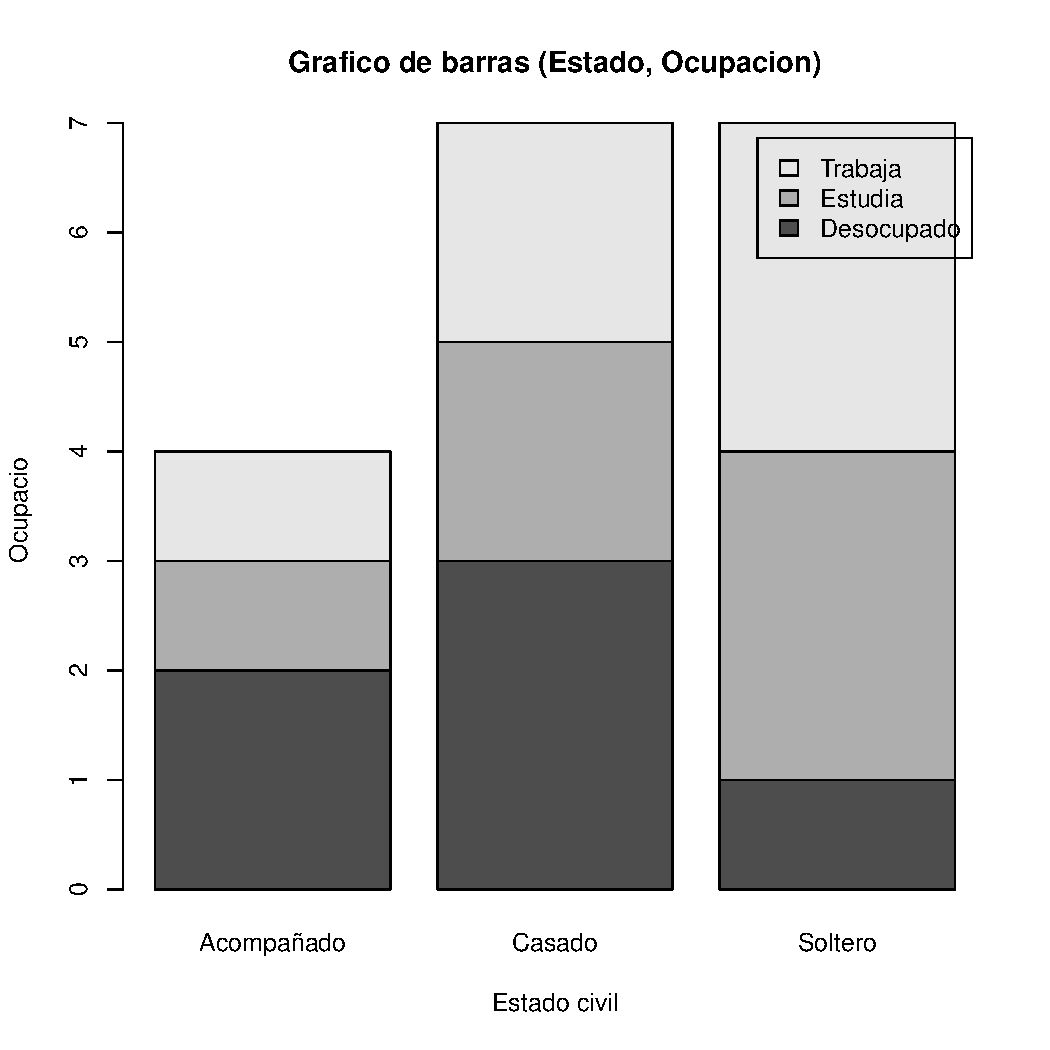
\includegraphics[width=\maxwidth]{figure/unnamed-chunk-1-1} 
\begin{kframe}\begin{alltt}
\hlkwd{barplot}\hlstd{(prop,} \hlkwc{main}\hlstd{=}\hlstr{"Gráfico de barras"}\hlstd{,} \hlkwc{xlab}\hlstd{=}\hlstr{" Consumo\textbackslash{}n"}\hlstd{,} \hlkwc{col}\hlstd{=}\hlkwd{c}\hlstd{(}\hlstr{"yellow"}\hlstd{,} \hlstr{"white"}\hlstd{,}\hlstr{"red"}\hlstd{),} \hlkwc{sub}\hlstd{=}\hlstr{"Agosto-2012"}\hlstd{)}
\end{alltt}
\end{kframe}
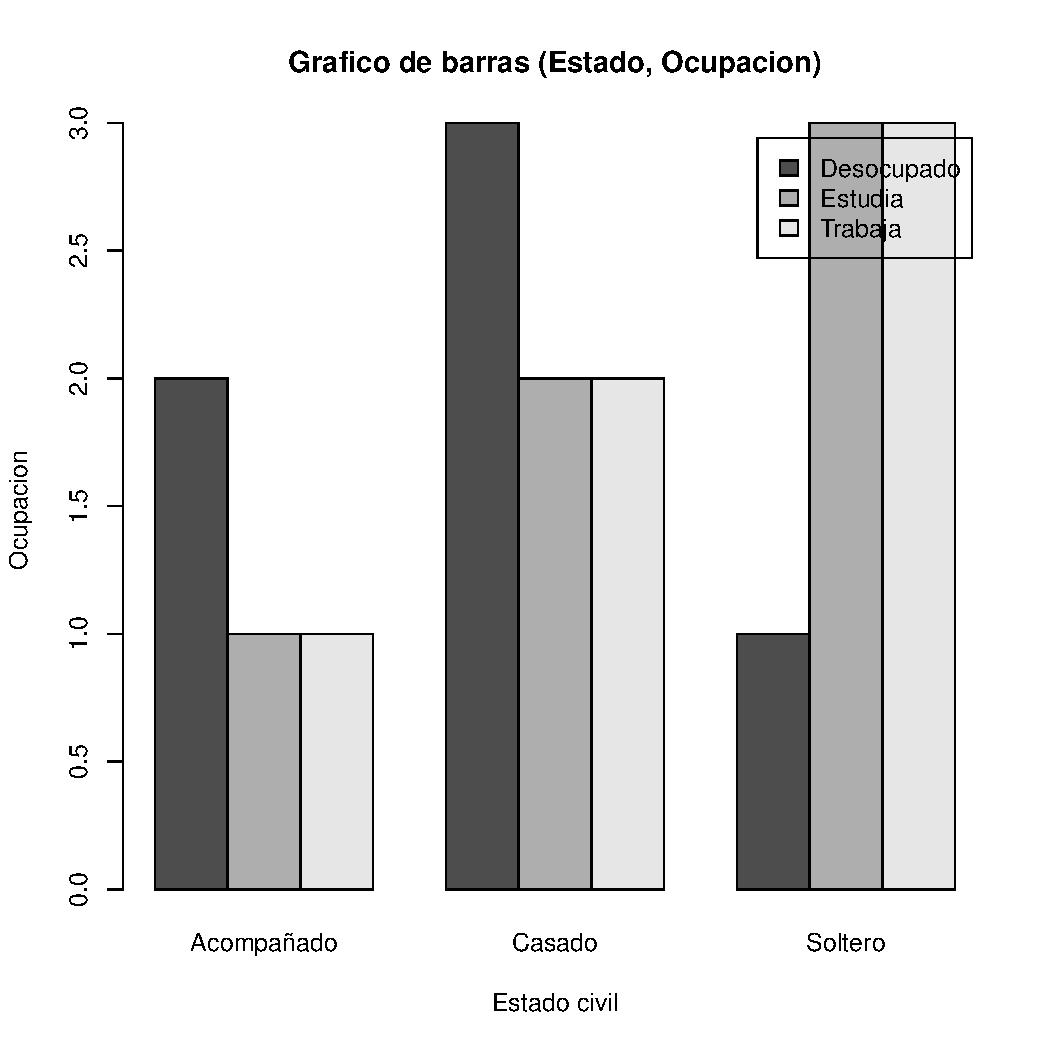
\includegraphics[width=\maxwidth]{figure/unnamed-chunk-1-2} 
\begin{kframe}\begin{alltt}
\hlkwd{pie}\hlstd{(frec,} \hlkwc{main}\hlstd{=}\hlstr{"Gráfico de pastel"}\hlstd{,} \hlkwc{xlab}\hlstd{=}\hlstr{"Tipo de Consumo"}\hlstd{,} \hlkwc{col}\hlstd{=}\hlkwd{c}\hlstd{(}\hlstr{"yellow"}\hlstd{,} \hlstr{"white"}\hlstd{,}\hlstr{"cyan"}\hlstd{),} \hlkwc{sub}\hlstd{=}\hlstr{"Agosto-2012"}\hlstd{)}
\end{alltt}
\end{kframe}
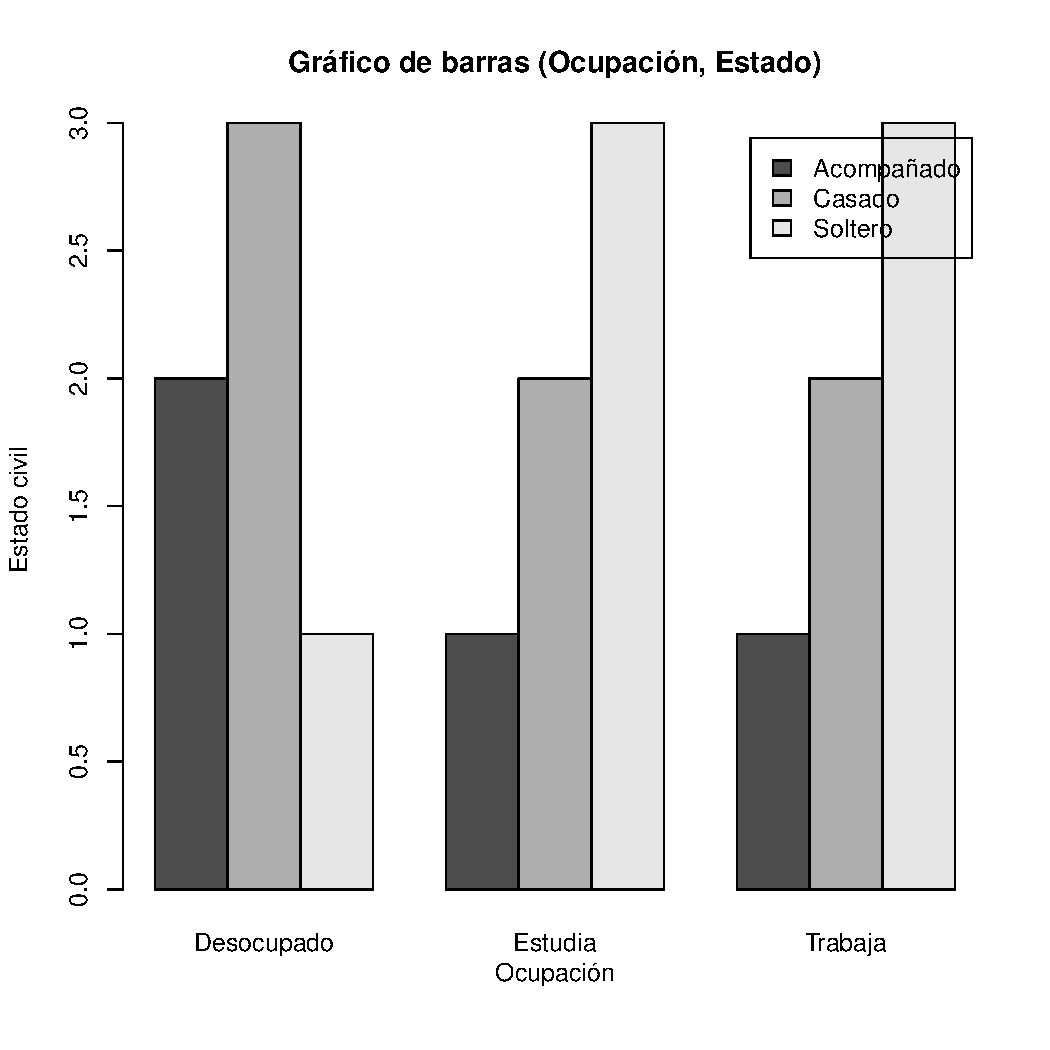
\includegraphics[width=\maxwidth]{figure/unnamed-chunk-1-3} 
\begin{kframe}\begin{alltt}
\hlkwd{names}\hlstd{(frec)} \hlkwb{=} \hlkwd{c}\hlstd{(}\hlstr{"Coca Cola"}\hlstd{,} \hlstr{"Pepsi"}\hlstd{,} \hlstr{"Salva Cola"}\hlstd{)}
\hlkwd{pie}\hlstd{(frec,} \hlkwc{main}\hlstd{=}\hlstr{"Gráfico de pastel"}\hlstd{,} \hlkwc{xlab}\hlstd{=}\hlstr{" Consumo"}\hlstd{,} \hlkwc{radius}\hlstd{=}\hlnum{0.8}\hlstd{,} \hlkwc{col}\hlstd{=}\hlkwd{c}\hlstd{(}\hlstr{"red"}\hlstd{,} \hlstr{"gray"}\hlstd{,}\hlstr{"cyan"}\hlstd{),} \hlkwc{sub}\hlstd{=}\hlstr{"Agosto-2012"}\hlstd{)}
\end{alltt}
\end{kframe}
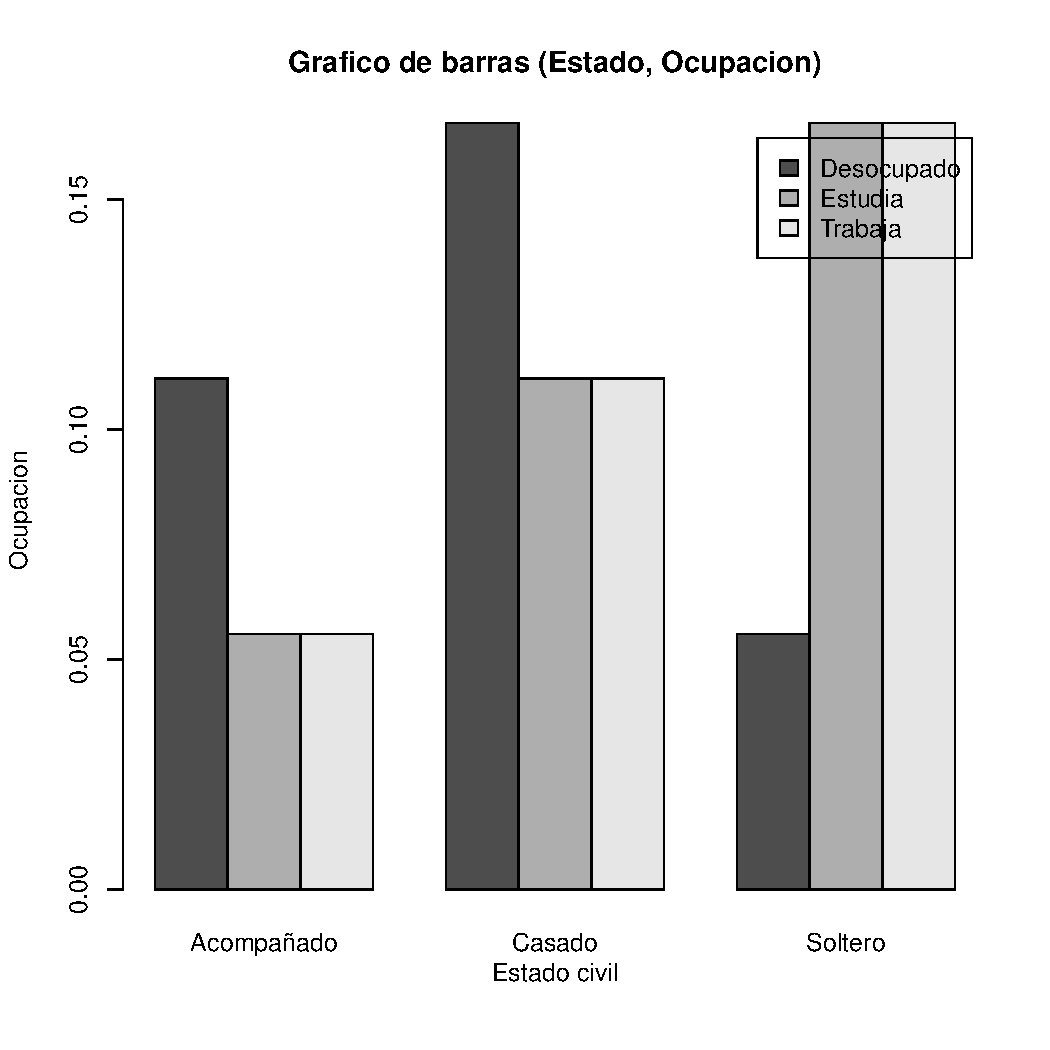
\includegraphics[width=\maxwidth]{figure/unnamed-chunk-1-4} 
\begin{kframe}\begin{alltt}
\hlstd{n} \hlkwb{<-} \hlkwd{length}\hlstd{(frec)}
\hlstd{hoja} \hlkwb{<-} \hlkwd{data.frame}\hlstd{(frec); hoja}
\end{alltt}
\begin{verbatim}
##         Var1 Freq
## 1  Coca Cola    4
## 2      Pepsi    8
## 3 Salva Cola    8
\end{verbatim}
\begin{alltt}
\hlstd{etiq} \hlkwb{<-} \hlkwd{c}\hlstd{(}\hlkwd{paste}\hlstd{(hoja}\hlopt{$}\hlstd{Var1,} \hlstr{"-"}\hlstd{, hoja}\hlopt{$}\hlstd{Freq)); etiq}
\end{alltt}
\begin{verbatim}
## [1] "Coca Cola - 4"  "Pepsi - 8"      "Salva Cola - 8"
\end{verbatim}
\begin{alltt}
\hlkwd{pie}\hlstd{(frec,} \hlkwc{main}\hlstd{=}\hlstr{"Gráfico de pastel"}\hlstd{,} \hlkwc{labels}\hlstd{=etiq,} \hlkwc{col}\hlstd{=}\hlkwd{rainbow}\hlstd{(n),} \hlkwc{border}\hlstd{=}\hlnum{TRUE}\hlstd{)}
\end{alltt}
\end{kframe}
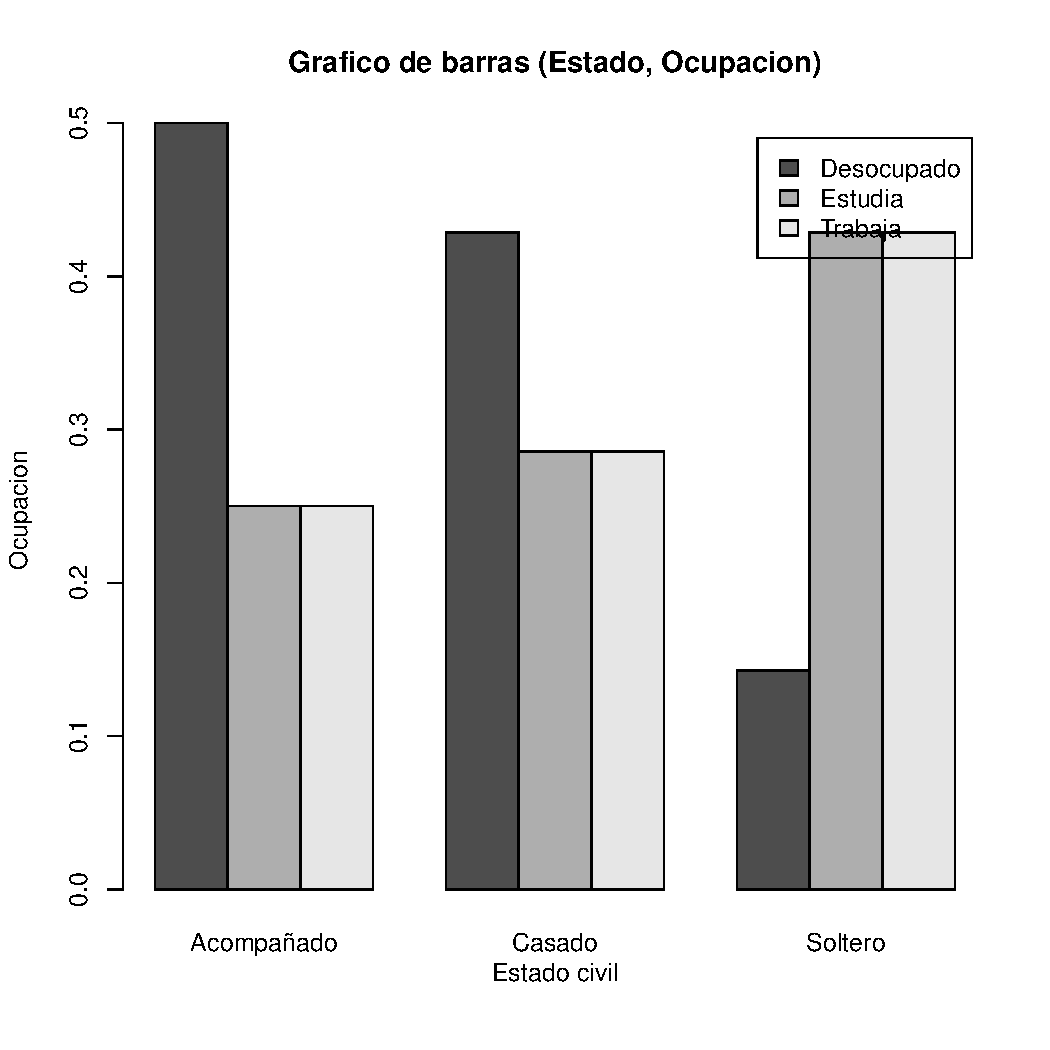
\includegraphics[width=\maxwidth]{figure/unnamed-chunk-1-5} 

\end{knitrout}



\end{document}
